\documentclass[11pt]{article}
\usepackage[utf8]{inputenc}

\usepackage{geometry}
\geometry{a4paper}

\usepackage{graphicx}
\usepackage{hyperref}
\usepackage[parfill]{parskip}
\usepackage{amsmath, amssymb}
\usepackage{fdsymbol}
\usepackage{color,soul}

% remove section numbering
\makeatletter
\renewcommand{\@seccntformat}[1]{}
\makeatother

% make subsubsection italic
\usepackage{sectsty}
\subsubsectionfont{\itshape}

\renewcommand{\arraystretch}{1.4}

\title{Probability Theory \& Statistics}
\date{}
\author{}

\begin{document}
\maketitle
\clearpage

\section{Counting}

\subsection{Prerequisites}

\begin{itemize}
\item
Events (and Naïve Probability)
\end{itemize}

\subsection{Introduction}

Calculating the naïve probability requires counting 
the number of outcomes in an event \(A\)
and counting the total number of outcomes in the sample space \(S\). 
In some problems it's possible to directly count these numbers with a \emph{combinatorial analysis}. 

\subsection{The Birthday Problem}

\subsubsection{Presentation}

Story problems are a useful way to remember collections of tools for solving problems. 
The \emph{birthday problem} uses several important tools from combinatorial
analysis and set theory to arrive at a quite surprising result.

Imagine a room with \(k\) people. 
We assume that each person's birthday is equally likely;
So no twins, triplets, ... and ignoring leap years.
Calculate the probability that two or more people in the room have the same birthday.

Attempt to solve the problem before reading the solution on the next page.

\clearpage
\subsubsection{Solution}

Since all the birthdays are equally likely, 
the naïve definition of probability applies, 
so that solving the problem is equivalent to
\begin{itemize}
\item
counting the total number of possible birthday combinations,
\item
then counting the number of outcomes where more than 2 people have the same birthday.
\end{itemize}

\emph{Multiplication rule}. 
For any compound experiment consisting of two sub-experiments, 
experiment A and experiment B. 
If experiment A has \(a\) possible outcomes, 
and experiment B has \(b\) possible outcomes,
then the compound experiment has \(ab\) possible outcomes and 
can be used to calculate the total number of possible outcomes.

\begin{figure}[h!]
\centering
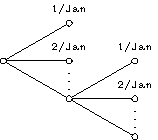
\includegraphics[width=0.25\linewidth]{tikz/figure1.pdf}
\caption{Tree representation of the birthday counting problem for \(k=2\) people.}
\label{fig:tree}
\end{figure}

For the birthday problem, 
each ``experiment'' corresponds to choosing one of the \(k\) people in the room. 
The number of (birthday) outcomes for each person is always the same -- 365. 
Since the number of outcomes is always the same for each person, 
we have a compounding experiment with \(365 \cdot 365 \ldots 365 = 365^k\) outcomes.
Figure \ref{fig:tree} represents the birthday problem as a series of 
branches for each experiment and its outcomes.

The total number of possible birthday combinations in a room of \(k\) people is an example 
of \emph{sampling with replacement}, 
where \(n\) is the number of things we're choosing from, 
and \(k\) is the number of times we choose something and then put it 
back in the pile of things to choose from.

For two people, 
we can directly calculate the probability of the event
that two people have the same birthday using the tree diagram 
-- the number of paths favourable to a match is 365, 
so that \(P\left( A_{2} \right) = 365/365^{2} = 1/365\). 
Equivalently,
we can assume the first chosen person knows his own birthday 
and there are 365 possible birthdays that the second person might have that match the first person's birthday, 
so a 1 in 365 chance of choosing the same birthday.%
\footnote{%
This approach requires a conditioning argument, 
\(P\left( A_{2} \right) = Q(A_{2}|B)\), 
where \(B\) is the event that each of them know their own birthday! 
Note that \emph{all probabilities} are conditional 
probabilities and conditional probabilities \emph{are probabilities!}}

Beyond two people, 
the counting problem becomes hard because it's difficult to count all the 
matches down each path of every tree, i.e.,
there could be a birthday match between either person 1 and 2, 
person 2 and 3, 
person 1 and 3, 
or all three (since the question asks for ``at least two matches'').

A (common) trick is to instead consider the complement of the event
that there are 2 or more people with the same birthday, i.e., 
what is the probability that nobody has the same birthday?

We again appeal to a common combinatorial tool, 
choosing \(k\) items from \(n\) objects \emph{without replacement} 
given by the following expression
\begin{align}
n \cdot (n - 1)\ldots(n - k + 1)
\end{align}
The reader is left to draw a corresponding tree diagram to explain why
this statement is true for counting the possible paths that result in no
birthday matches.

Finally, 
from the naïve definition of probability and the fact that
\(P\left( \overline{A} \right) = 1 - P(A)\), we arrive at the desired result
\begin{align}
P\left( A_{k} \right) = 1 - \frac{365\cdot(365 - 1)\ldots(365 - k + 1)}{365^{k}}
\end{align}
Evaluating the above expression shows that the probability of a match is
greater than 50\% for a room with 23 people. 

It seems surprisingly probable that at least two people have the same birthday for so few people. 
However, 
the result can be explained by calculating the 
number of \emph{pairs of people} in a room of \(k\) people. 

The number of pairs of
people is given by the \emph{binomial coefficient}
\begin{align}
C_{k}^{n} = \binom{n}{k} = \frac{n\cdot(n-1)\ldots(n-k+1)}{k\cdot(k-1)\ldots 1} = \frac{n!}{k!(n - k)!}.
\end{align}
For \(n = 23\), 
and \(k = 2\), 
we have 253 possibilities of a potential match. 
So even though there is a low probability of any \emph{single pair} matching, 
there are many \emph{combinations of people} from which to draw potential matches.

\clearpage
\section{Practice}

1) In the birthday problem we described three combinatorial 
tools summarized in the following table.

\begin{table}[h!]
\centering
\begin{tabular}{| r | c | c |}
\hline
 & Ordered & Unordered \\\hline
Replacement & \(n^{k}\) & ? \\\hline
Without Replacement  & \(n\cdot (n-1) \ldots (n-k+1)\) & \(C_{k}^{n}\) \\\hline
\end{tabular}
\caption{%
Summary table of combinatorial counting expressions.
}
\end{table}

Show that the expression for sampling unordered \(k\)-groups from \(n\) objects is 
given by solving the isomorphic problem of putting \(k\) indistinguishable particles 
into \(n\) distinguishable boxes.

2) What is the probability that there are exactly \(k\) birthday matches (as opposed to at least \(k\) matches)?

3) Is the probability that there are at least two people with the same birthday less than, 
greater than, 
or equal to the same event for birthdays that aren't equally likely? 
For example, 
if there are \(m\) twins in the room.

\section{Appendix}

\subsection{Lists}

A reminder about ordered and unordered lists or \(k\)-groups. 
Consider the set \(A = \{a,b,c\}\) containing \(n=3\) elements.
Choosing \emph{ordered} \(2\)-groups \emph{with replacement} we have: 
\(ab\), \(ba\), \(ac\), \(ca\), \(bc\), \(cb\), \(aa\), \(bb\), and \(cc\). 
Thus there are \(n^{k} = 3^2 = 9\) ways to choose an ordered 2-group 
with replacement from three objects.

\emph{Unordered} \(k\)-groups mean that the 2-groups \(ab\) and \(ba\) are the same. 
The unordered 2-group \emph{with replacement} for three objects is: 
\(ab\), \(ac\), \(bc\), \(aa\), \(bb\), and \(cc\).
Fewer than the ordered case.

Choosing \(2\)-groups \emph{without replacement} means we can't choose items
that have already been picked, 
so the 2-groups \(aa\), \(bb\), and \(cc\) aren't included in either the ordered or unordered cases.

\subsection{Binomial Coefficient}

The binomial coefficient is the final combinatorial tool of this problem. 
We are asked to calculate the number of ways to choose couples (two people) from 23 people. 
Recall that the number of ways to choose \(k\) \emph{ordered} items 
from \(n\) objects \emph{without replacement} is given by
\begin{align}
n\cdot(n - 1)\ldots(n - k + 1).
\end{align}
In the context of the problem, 
we can imagine that the 23 people are labelled and standing in a line. 
We choose the first person out of the 23 people in the line. 
We then match that person to each of the remaining people left in the pool of 22 people, 
of which there are 22 possible choices. 
Since we could have chosen any of the 23 people as the first person, 
we have \(23\cdot(23 - 1)\) possible couples. 
This is equivalent to choosing 2-groups from 23 objects without replacement and 
agrees with the expression for \(n=23\) and \(k=2\).

This calculation however overcounts since by taking 23 possible choices for the first person, 
we must have inadvertently chosen the other person in the couple,
doubling counting since we are only interested unordered pairs.
By the multiplication (and division) rule, 
we can account for the overcount by dividing the total number of couples (accounting for order) 
by the number of ways we can order the couples, i.e., \(2!\), 
yielding the binomial coefficient for groups of size \(k = 2\). 
The general expression follows by induction.

\end{document}
